\documentclass{article}
\usepackage{tikz, comment}
\usepackage{pifont}
\usepackage{fontspec}
\usetikzlibrary{arrows, decorations.markings, decorations.pathreplacing}
\begin{comment}
:Title: Not defined yet
:Tags: aa similarity;aas congruence, saa congruence ;abscissa;absolute convergence, absolutely convergent ;absolute maximum, absolute max, global maximum, global max
:Prob: nan;nan;nan;nan;nan
:Author: Prof.Hu Ji-shan, HKUST
:Slug: No name yet

Description Here.........
\end{comment}
\begin{document}\centering

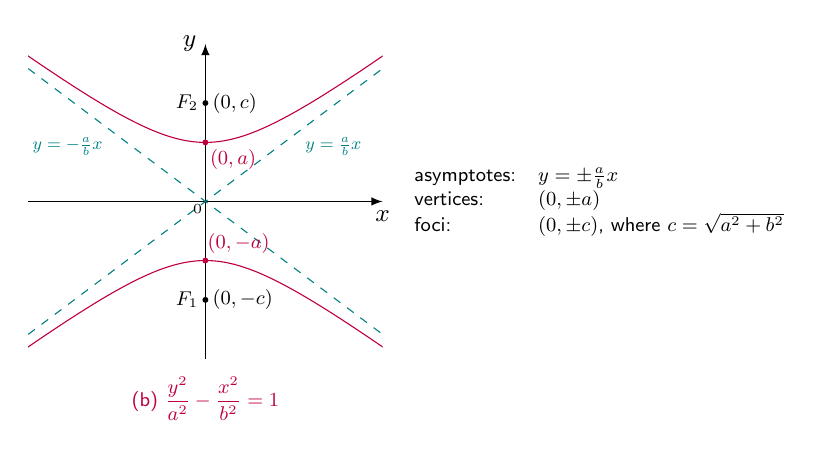
\begin{tikzpicture}[>=latex,xscale=.5*0.5, yscale=.5*0.5][font=\sf\small]

\draw[->] (-9, 0) -- (9, 0)node[below] {\small $x$};
\draw[->] (0, -8) -- (0, 8)node[left] {\small $y$};

\node[purple, scale=0.8] at (0, -10) {(b) $\displaystyle \frac{y^2}{a^2}-\frac{x^2}{b^2}=1$};

\node[scale=0.8] at (20, 0) {$
\begin{array}{ll}
\hbox{asymptotes:} & y = \pm \frac{a}{b}x \\
\hbox{vertices:} & (0, \pm a) \\
\hbox{foci:} & \hbox{$(0, \pm c)$, where $c = \sqrt{a^2+b^2}$}
\end{array}
$};

\clip[] (-9,-8) rectangle (9,8);

\draw[teal, dashed, samples=100, smooth, domain=-9:9, variable=\x]
plot ({\x}, {-3/4*(\x)});
\draw[teal, dashed, samples=100, smooth, domain=-9:9, variable=\x]
plot ({\x}, { 3/4*(\x)});
\node[teal, scale=0.7] at (-7, 2.8) {$y = -\frac{a}{b}x$};
\node[teal, scale=0.7] at ( 6.5, 2.8) {$y = \frac{a}{b}x$};

\draw[purple, samples=100, smooth, domain=-2:2, variable=\t]
plot ({4*sinh(\t)}, {3*cosh(\t)}) ;

\draw[purple, samples=100, smooth, domain=-3:3, variable=\t]
plot ({4*sinh(\t)}, {-3*cosh(\t)}) ;

\draw[fill, xscale=1/0.5, yscale=1/0.5] (0, -5*0.5) circle(0.06) node[left, scale=0.8]{$F_1$} node[right, scale=0.8]{$(0,-c)$};
\draw[fill, xscale=1/0.5, yscale=1/0.5] (0, 5*0.5) circle(0.06) node[left, scale=0.8]{$F_2$} node[right, scale=0.8]{$(0, c)$};

\draw[purple, fill, xscale=1/0.5, yscale=1/0.5] (0, 3*0.5) circle(0.06) node[below, xshift=10, scale=0.8]{$(0, a)$};
\draw[purple, fill, xscale=1/0.5, yscale=1/0.5] (0,-3*0.5) circle(0.06) node[above, xshift=12, scale=0.8]{$(0, -a)$};

\node at (-0.2/0.5, -0.2/0.5) {\tiny$0$};

\end{tikzpicture}
\end{document}